\chapter{Методы защиты информации} \label{chapt2}%
\textbf{Мета роботи:~}%
На практике использовать основные методы криптографической зашиты информации.
\section{Теоретические ведомости} \label{sect8_a}
%
Появление новых информационных технологий и развитие мощных компьютерных
систем хранения и обработки информации повысили уровни защиты информации и
вызвали необходимость того, чтобы эффективность защиты информации росла
вместе со сложностью архитектуры хранения данных. Постепенно защита
информации становится обязательной: разрабатываются всевозможные документы по
защите информации; формируются рекомендации; даже проводится ФЗ о защите
информации, который рассматривает проблемы и задачи защиты информации, а
также решает некоторые уникальные вопросы защиты информации.

Таким образом, угроза защиты информации сделала средства обеспечения
информационной безопасности одной из обязательных характеристик
информационной системы.

\begin{figure}[h]
  \centering
  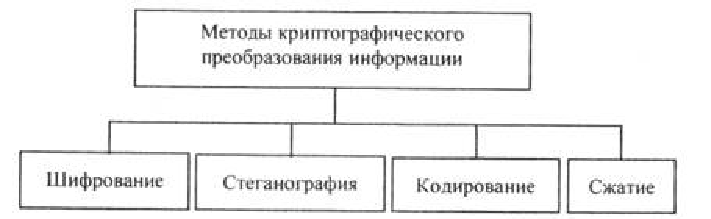
\includegraphics[width=\linewidth]{img2_1.pdf}
  \caption{Методы криптографического преобразования информации}\label{img:img2_1}
\end{figure}



\subsection{Симметричные криптосистемы}
\subsubsection{Шифры перестановки}
В шифрах средних веков часто использовались таблицы, с помощью которых
выполнялись простые процедуры шифрования, основанные на перестановке букв в
сообщении. Ключом в данном случае является размеры таблицы. Например,
сообщение <<Неясное становится ещё более непонятным>> записывается в таблицу
из 5 строк и 7 столбцов по столбцам.

\begin{table} [htbp]% Пример записи таблицы с номером, но без отображаемого наименования
  \centering
  \parbox{6cm}{% чтобы лучше смотрелось, подбирается самостоятельно
    \captiondelim{}% должен стоять до самого пустого caption
    \caption{}%
    \label{tabl:tab2x1}%
    \begin{SingleSpace}
      \begin{tabular}{ | c | c | c | c | c | c | c |}
        \hline
          Н & О & Н & С & Б & Н & Я \\ \hline
          Е & Е & О & Я & О & Е & Т \\ \hline
          Я & С & В & Е & Л & П & Н \\ \hline
          С & Т & И & Щ & Е & О & Ы \\ \hline
          Н & А & Т & Ё & Е & Н & М \\ \hline
      \end{tabular}%
    \end{SingleSpace}
  }
\end{table}
Для получения шифрованного сообщения текст считывается по строкам и
группируется по 5 букв:
\begin{center}
НОНСБ--НЯЕЕО--ЯОЕТЯ--СВЕЛП--НСТИЩ--ЕОЫНА--ТЕЕНМ
\end{center}

Несколько большей стойкостью к раскрытию обладает метод \emph{одиночной
перестановки} по ключу. Он отличается от предыдущего тем, что столбцы таблицы
переставляются по ключевому слову, фразе или набору чисел длиной в строку
таблицы. Используя в качестве ключа слово - \texttt{ЛУНАТИК}, получим
следующую таблицу:

\begin{table} [htbp]% Пример записи таблицы с номером, но без отображаемого наименования
  \centering
  \parbox{12cm}%
  {% чтобы лучше смотрелось, подбирается самостоятельно
    \caption{Метод перестановки по ключу}%
    \label{tabl:tab2x2}%
    \begin{SingleSpace}
      \begin{tabular}{ccccccccccccccc}
      \cline{1-7} \cline{9-15}
      \multicolumn{1}{|c|}{{\ul Л}}    & \multicolumn{1}{c|}{{\ul У}}    & \multicolumn{1}{c|}{{\ul Н}}    & \multicolumn{1}{c|}{{\ul А}}    & \multicolumn{1}{c|}{{\ul Т}}    & \multicolumn{1}{c|}{{\ul И}}    & \multicolumn{1}{c|}{{\ul К}}    & \multicolumn{1}{c|}{} & \multicolumn{1}{c|}{{\ul А}}    & \multicolumn{1}{c|}{{\ul И}}    & \multicolumn{1}{c|}{{\ul К}}    & \multicolumn{1}{c|}{{\ul Л}}    & \multicolumn{1}{c|}{{\ul Н}}    & \multicolumn{1}{c|}{{\ul Т}}    & \multicolumn{1}{c|}{{\ul У}}    \\ \cline{1-7} \cline{9-15}
      \multicolumn{1}{|c|}{\textbf{4}} & \multicolumn{1}{c|}{\textbf{7}} & \multicolumn{1}{c|}{\textbf{5}} & \multicolumn{1}{c|}{\textbf{1}} & \multicolumn{1}{c|}{\textbf{6}} & \multicolumn{1}{c|}{\textbf{2}} & \multicolumn{1}{c|}{\textbf{3}} & \multicolumn{1}{c|}{} & \multicolumn{1}{c|}{\textbf{1}} & \multicolumn{1}{c|}{\textbf{2}} & \multicolumn{1}{c|}{\textbf{3}} & \multicolumn{1}{c|}{\textbf{4}} & \multicolumn{1}{c|}{\textbf{5}} & \multicolumn{1}{c|}{\textbf{6}} & \multicolumn{1}{c|}{\textbf{7}} \\ \cline{1-7} \cline{9-15}
      \multicolumn{1}{|c|}{Н}          & \multicolumn{1}{c|}{О}          & \multicolumn{1}{c|}{Н}          & \multicolumn{1}{c|}{С}          & \multicolumn{1}{c|}{Б}          & \multicolumn{1}{c|}{Н}          & \multicolumn{1}{c|}{Я}          & \multicolumn{1}{c|}{} & \multicolumn{1}{c|}{С}          & \multicolumn{1}{c|}{Н}          & \multicolumn{1}{c|}{Я}          & \multicolumn{1}{c|}{Н}          & \multicolumn{1}{c|}{Н}          & \multicolumn{1}{c|}{Б}          & \multicolumn{1}{c|}{О}          \\ \cline{1-7} \cline{9-15}
      \multicolumn{1}{|c|}{Е}          & \multicolumn{1}{c|}{Е}          & \multicolumn{1}{c|}{О}          & \multicolumn{1}{c|}{Я}          & \multicolumn{1}{c|}{О}          & \multicolumn{1}{c|}{Е}          & \multicolumn{1}{c|}{Т}          & \multicolumn{1}{c|}{} & \multicolumn{1}{c|}{Я}          & \multicolumn{1}{c|}{Е}          & \multicolumn{1}{c|}{Т}          & \multicolumn{1}{c|}{Е}          & \multicolumn{1}{c|}{О}          & \multicolumn{1}{c|}{О}          & \multicolumn{1}{c|}{Е}          \\ \cline{1-7} \cline{9-15}
      \multicolumn{1}{|c|}{Я}          & \multicolumn{1}{c|}{С}          & \multicolumn{1}{c|}{В}          & \multicolumn{1}{c|}{Е}          & \multicolumn{1}{c|}{Л}          & \multicolumn{1}{c|}{П}          & \multicolumn{1}{c|}{Н}          & \multicolumn{1}{c|}{} & \multicolumn{1}{c|}{Е}          & \multicolumn{1}{c|}{П}          & \multicolumn{1}{c|}{Н}          & \multicolumn{1}{c|}{Я}          & \multicolumn{1}{c|}{В}          & \multicolumn{1}{c|}{Л}          & \multicolumn{1}{c|}{С}          \\ \cline{1-7} \cline{9-15}
      \multicolumn{1}{|c|}{С}          & \multicolumn{1}{c|}{Т}          & \multicolumn{1}{c|}{И}          & \multicolumn{1}{c|}{Щ}          & \multicolumn{1}{c|}{Е}          & \multicolumn{1}{c|}{О}          & \multicolumn{1}{c|}{Ы}          & \multicolumn{1}{c|}{} & \multicolumn{1}{c|}{Щ}          & \multicolumn{1}{c|}{О}          & \multicolumn{1}{c|}{Ы}          & \multicolumn{1}{c|}{С}          & \multicolumn{1}{c|}{И}          & \multicolumn{1}{c|}{Е}          & \multicolumn{1}{c|}{Т}          \\ \cline{1-7} \cline{9-15}
      \multicolumn{1}{|c|}{Н}          & \multicolumn{1}{c|}{А}          & \multicolumn{1}{c|}{Т}          & \multicolumn{1}{c|}{Е}          & \multicolumn{1}{c|}{Е}          & \multicolumn{1}{c|}{Н}          & \multicolumn{1}{c|}{М}          & \multicolumn{1}{c|}{} & \multicolumn{1}{c|}{Е}          & \multicolumn{1}{c|}{Н}          & \multicolumn{1}{c|}{М}          & \multicolumn{1}{c|}{Н}          & \multicolumn{1}{c|}{Т}          & \multicolumn{1}{c|}{Е}          & \multicolumn{1}{c|}{А}          \\ \cline{1-7} \cline{9-15}
      \multicolumn{7}{c}{До перестановки}                                                                                                                                                                                                          & \multicolumn{1}{l}{}  & \multicolumn{7}{c}{После перестановки}
      \end{tabular}
    \end{SingleSpace}
  }
\end{table}

В верхней строке левой таблицы записан ключ, а номера под буквами ключа
определены в соответствии с естественным порядком соответствующих букв ключа
в алфавите. Если в ключе встретились бы одинаковые буквы, они бы нумеровались
слева направо. Получается шифровка:%
\begin{center}
СНЯНН--БОЯЕТ--ЕООЕЕ--ПНЯВЛ--СЩОЫС--ИЕТЕН--МНТЕА
\end{center}

Для обеспечения дополнительной скрытности можно повторно шифровать сообщение,
которое уже было зашифровано. Для этого размер второй таблицы подбирают так,
чтобы длины её строк и столбцов отличались от длин строк и столбцов первой
таблицы. Лучше всего, если они будут взаимно простыми.

Кроме алгоритмов одиночных перестановок применяются алгоритмы двойных
перестановок. Сначала в таблицу записывается текст сообщения, а потом
поочередно переставляются столбцы, а затем строки. При расшифровке порядок
перестановок был обратный. Пример данного метода шифрования показан в таблице
\ref{tabl:tab2x3}.

\begin{table} [htbp]% Пример записи таблицы с номером, но без отображаемого наименования
  \centering
  \parbox{12cm}{% чтобы лучше смотрелось, подбирается самостоятельно
    \caption{Метод перестановки по ключу}%
    \label{tabl:tab2x3}%
    \begin{SingleSpace}
      \begin{tabular}{c|c|c|c|c|cc|c|c|c|c|cc|c|c|c|c|}
      \cline{2-5} \cline{8-11} \cline{14-17}
      \textbf{}                        & \textbf{2}                                                & \textbf{4} & \textbf{1} & \textbf{3}                                                &                       & \textbf{} & {\color[HTML]{00FE00} \textbf{1}} & {\color[HTML]{00FE00} \textbf{2}}                         & {\color[HTML]{00FE00} \textbf{3}}                         & {\color[HTML]{00FE00} \textbf{4}} &                       &                                   & 1 & 2                                                         & 3                                                         & 4 \\ \cline{1-5} \cline{7-11} \cline{13-17}
      \multicolumn{1}{|c|}{\textbf{4}} & \cellcolor[HTML]{ECF4FF}{\color[HTML]{000000} \textbf{П}} & Р          & И          & Е                                                         & \multicolumn{1}{c|}{} & 4         & И                                 & \cellcolor[HTML]{ECF4FF}{\color[HTML]{000000} \textbf{П}} & Е                                                         & Р                                 & \multicolumn{1}{c|}{} & {\color[HTML]{FE0000} \textbf{1}} & А & З                                                         & Ю                                                         & Ж \\ \cline{1-5} \cline{7-11} \cline{13-17}
      \multicolumn{1}{|c|}{\textbf{1}} & З                                                         & Ж          & А          & Ю                                                         & \multicolumn{1}{c|}{} & 1         & А                                 & 3                                                         & Ю                                                         & Ж                                 & \multicolumn{1}{c|}{} & {\color[HTML]{FE0000} \textbf{2}} & Е & -                                                         & С                                                         & Ш \\ \cline{1-5} \cline{7-11} \cline{13-17}
      \multicolumn{1}{|c|}{\textbf{2}} & -                                                         & Ш          & Е          & С                                                         & \multicolumn{1}{c|}{} & 2         & Е                                 & -                                                         & С                                                         & Ш                                 & \multicolumn{1}{c|}{} & {\color[HTML]{FE0000} \textbf{3}} & Г & Т                                                         & \cellcolor[HTML]{ECF4FF}{\color[HTML]{000000} \textbf{О}} & О \\ \cline{1-5} \cline{7-11} \cline{13-17}
      \multicolumn{1}{|c|}{\textbf{3}} & Т                                                         & О          & Г          & \cellcolor[HTML]{ECF4FF}{\color[HTML]{000000} \textbf{О}} & \multicolumn{1}{c|}{} & 3         & Г                                 & Т                                                         & \cellcolor[HTML]{ECF4FF}{\color[HTML]{000000} \textbf{О}} & О                                 & \multicolumn{1}{c|}{} & {\color[HTML]{FE0000} \textbf{4}} & И & \cellcolor[HTML]{ECF4FF}{\color[HTML]{000000} \textbf{П}} & Е                                                         & Р \\ \cline{1-5} \cline{7-11} \cline{13-17}
      \end{tabular}
    \end{SingleSpace}
  }
\end{table}
Ключом к шифру служат номера столбцов \textbf{\textcolor[rgb]{0,1,0}{2413}} и
номера строк \textbf{\textcolor[rgb]{1,0,0}{4123}} исходной таблицы. В
результате перестановки получена шифровка:
\begin{center}
АЗЮЖЕ\_СШГТООИПЕР
\end{center}
Число вариантов двойной перестановки достаточно быстро возрастает с
увеличением размера таблицы: для таблицы $3 х 3$ их $36$, для $4 х 4$ их
$576$, а для $5\cdot 5$ их $14400$.

В средние века для шифрования применялись и магические квадраты. Магическими
квадратами называются квадратные таблицы с вписанными в их клетки
последовательными натуральными числами, начиная с единицы, которые дают в
сумме по каждому столбцу, каждой строке и каждой диагонали одно и то же
число. Для шифрования необходимо вписать исходный текст по приведённой в
квадрате нумерации и затем переписать содержимое таблицы по строкам.
\begin{table} [htbp]% Пример записи таблицы с номером, но без отображаемого наименования
  \centering
  \parbox{14cm}{% чтобы лучше смотрелось, подбирается самостоятельно
    \caption{Исходный текст с идентификаторами}%
    \label{tabl:tab2x4}%
    \begin{SingleSpace}
\begin{tabular}{c|c|c|c|c|c|c|c|c|c|c|c|c|c|c|c}
П & Р & И & Е & З & Ж & А & Ю & \_ & Ш & Е & С & Т & О & Г & О \\ \hline
1 & 2 & 3 & 4 & 5 & 6 & 7 & 8 & 9 & 10 & 11 & 12 & 13 & 14 & 15 & 16 \\
\end{tabular}
    \end{SingleSpace}
  }
\end{table}
\begin{table}% Пример записи таблицы с номером, но без отображаемого наименования
  \centering
  \parbox{10cm}{% чтобы лучше смотрелось, подбирается самостоятельно
    \caption{Магический квадрат}%
    \label{tabl:tab2x5}%
    \begin{SingleSpace}
      \begin{tabular}{|c|c|c|c|c|c|c|c|c|}
\cline{1-4} \cline{6-9}
16 & 3  & 2  & 13 &                     & О & И & Р & Т \\ \cline{1-4} \cline{6-9}
5  & 10 & 11 & 8  & {\Huge $\dashrightarrow$} & З & Ш & Е & Ю \\ \cline{1-4} \cline{6-9}
9  & 6  & 7  & 12 & {\Huge $\dashleftarrow$}  & - & Ж & А & С \\ \cline{1-4} \cline{6-9}
4  & 15 & 14 & 1  &                     & Е & Г & О & П \\ \cline{1-4} \cline{6-9}
      \end{tabular}
    \end{SingleSpace}
  }
\end{table}
В результате получается шифротекст, сформированный благодаря перестановке
букв исходного сообщения.

Число магических квадратов очень резко возрастает с увеличением размера его
сторон: для таблицы $3\times 3~\Rightarrow~1$ существует только один квадрат;
для таблицы $4\times 4~\Rightarrow~880$; а для таблицы $5\times
5~\Rightarrow~250 000$.


\subsubsection{Шифры простой замены}

\subparagraph{Система шифрования Цезаря} частный случай шифра простой замены.
Метод основан на замене каждой буквы сообщения на другую букву того же
алфавита, путем смещения от исходной буквы на \emph{K} букв. Известная фраза
Юлия Цезаря \texttt{VENI VINI VICI} – пришел, увидел, победил, зашифрованная
с помощью данного метода, преобразуется в \texttt{SBKF SFAF SFZF} (при
смещении на 4 символа). Греческим писателем Полибием за 100 лет до н.э. был
изобретён так называемый полибианский квадрат размером $5\times 5$,
заполненный алфавитом в случайном порядке. Греческий алфавит имеет 24 буквы,
а 25-м символом является пробел. Для шифрования на квадрате находили букву
текста и записывали в шифротекст букву, расположенную ниже её в том же
столбце. Если буква оказывалась в нижней строке таблицы, то брали верхнюю
букву из того же столбца.

\subsubsection{Шифры сложной замены}

\subparagraph{Шифр Гронсфельда} состоит в модификации шифра Цезаря числовым
ключом. Для этого под буквами сообщения записывают цифры числового ключа.
Если ключ короче сообщения, то его запись циклически повторяют. Шифротекст
получают примерно так же, как в шифре Цезаря, но отсчитывают не третью букву
по алфавиту (как в шифре Цезаря), а ту, которая смещена по алфавиту на
соответствующую цифру ключа.
\begin{Notes}
  \item пусть в качестве ключа используется группа из трех цифр - 314;
  \item тогда Сообщение СОВЕРШЕННО СЕКРЕТНО;
  \item Ключ 3143143143143143143;
  \item Шифровка ФПЖИСЬИОССАХИЛФИУСС.
\end{Notes}
В шифрах \emph{многоалфавитной замены} для шифрования каждого символа
исходного сообщения применяется свой шифр простой замены (свой алфавит).

В компьютере операция шифрования соответствует сложению кодов ASCII символов
сообщения и ключа по модулю 256.

\subsubsection{Гаммирование}
Процесс зашифрования заключается в генерации гаммы шифра и наложении этой
гаммы на исходный открытый текст. Перед шифрованием открытые данные
разбиваются на блоки $T(0)_i$ одинаковой длины (по 64 бита). Гамма шифра
вырабатывается в виде последовательности блоков Г(c)i аналогичной длины
$Т(c)_i=G(c)_i \oplus T(0)_i$, где $\oplus $ - побитовое сложение, $i =1-m$).

Процесс расшифрования сводится к повторной генерации шифра текста и наложение
этой гаммы на зашифрованные данные $T(0)_i=G(c)_i\oplus Т(c)_i$.

Исходное сообщение из букв русского алфавита преобразуется в числовое
сообщение заменой каждой его буквы числом по следующей таблице:


\begin{table}[htbp]% Пример записи таблицы с номером, но без отображаемого наименования
  \centering
  \caption{Числовая замена букв}%
  \label{tabl:tab2x6}%
    \begin{SingleSpace}
    \begin{tabularx}{\textwidth}{|C|C|C|C|C|C|C|C|C|C|C|C|C|C|C|}
      \hline
      А  & Б  & В  & Г  & Д  & Е  & Ж  & З  & И  & К  & Л  & М  & Н  & О  & П  \tabularnewline \hline
      00 & 01 & 02 & 03 & 04 & 05 & 06 & 07 & 08 & 09 & 10 & 11 & 12 & 13 & 14 \tabularnewline \hline
      Р  & С  & Т  & У  & Ф  & Х  & Ц  & Ч  & Ш  & Щ  & Ь  & Ы  & Э  & Ю  & Я  \tabularnewline \hline
      15 & 16 & 17 & 18 & 19 & 20 & 21 & 22 & 23 & 24 & 25 & 26 & 27 & 28 & 29 \tabularnewline \hline
      \end{tabularx}
  \end{SingleSpace}
\end{table}
\begin{equation}\label{formul:fml2_1}
  {\Omega}_{i+1}= [(A_i + C_1 – 1)\cdot mod30] + 1;
\end{equation}

Исходное сообщение ОТДУШКА. Для шифрования числового сообщения используется
шифрующий отрезок последовательности А1, А2, ... подходящей длины,
начинающийся с $A_{100}$: $A_{101}\rightarrow 5$, $A_{102}\rightarrow 6$,
$A_{103}\rightarrow 17$, $A_{104}\rightarrow 18$, $A_{105}\rightarrow 19$,
$A_{106}\rightarrow 3$.

\begin{table}[htbp]% Пример записи таблицы с номером, но без отображаемого наименования
  \centering
    \captiondelim{}% должен стоять до самого пустого caption
  %\caption{}%caption{Пример шифрования методом гаммирование}%
  \label{tabl:tab2x7}%
  \begin{tabular}{lccccccc}
    Исходное сообщение             & О  & Т  & Д  & У  & Ш  & К  & А \\
    \rowcolor[HTML]{EFEFEF}
    Числовое исходное сообщение    & 13 & 17 & 4  & 18 & 23 & 9  & 0 \\
    Шифрующий отрезок              & 1  & 5  & 6  & 17 & 8  & 19 & 3 \\
    \rowcolor[HTML]{EFEFEF}
    Числовое шифрованное сообщение & 14 & 23 & 10 & 5  & 1  & 28 & 3 \\
    Шифрованное сообщение          & П  & Ш  & Л  & Е  & Б  & Ю  & Г
  \end{tabular}
\end{table}

\section{Задания}\label{sect8_b}
%
(из заданий к экзамену)
\section{Пример выполнения работы}\label{sect8_c}
%
\section{Варианты}\label{sect8_d}
%
\section{Вопросы для контроля}\label{sect8_e}
%
\begin{enumerate}
  \item
  \item
  \item
\end{enumerate}
